\documentclass[a4paper]{jpconf}

\usepackage{hyperref}
\usepackage{graphicx}
\usepackage{bm}        % for math
\usepackage{amssymb}   % for math
\usepackage{amsfonts}
\usepackage{amsmath}
\usepackage{epsfig}
\usepackage{units}
\usepackage{cite}
%\usepackage[numbers,square,sort&compress]{natbib}
\usepackage[utf8]{inputenc}
\usepackage[T1]{fontenc}

%particles
\newcommand{\jpsi}{\rm J/$\psi$}
\newcommand{\psip}{$\psi^\prime$}
\newcommand{\jpsiDY}{\rm J/$\psi$\,/\,DY}
\newcommand{\chic}{$\chi_{\rm c}$}
\newcommand{\pip}{$\pi^{+}$}
\newcommand{\pim}{$\pi^{-}$}
\newcommand{\pizero}{$\pi^{0}$}
\newcommand{\kap}{K$^{+}$}
\newcommand{\kam}{K$^{-}$}
\newcommand{\pbar}{$\rm\overline{p}$}
\newcommand{\ccbar}{\ensuremath{\mathrm{c\overline{c}}}}
\newcommand{\bbbar}{\ensuremath{\mathrm{b\overline{b}}}}
\newcommand{\Dzero}{\ensuremath{\mathrm{D^{0}}}}
\newcommand{\Dzerobar}{\ensuremath{\mathrm{\overline{D}^{0}}}}
\newcommand{\Dpm}{\ensuremath{\mathrm{D^{\pm}}}}
\newcommand{\Ds}{\ensuremath{\mathrm{D_{s}^{\pm}}}}
\newcommand{\Dstar}{\ensuremath{\mathrm{D^{*\pm}}}}

%collision systems
\newcommand{\pp}{pp}
\newcommand{\pPb}{p--Pb}
\newcommand{\PbPb}{Pb--Pb}

%detectors
\newcommand{\ezdc}{$E_{\rm ZDC}$}

%units
\newcommand{\GeVc}{GeV/$c$}
\newcommand{\GeVcsq}{GeV/$c^2$}

%others
\newcommand{\degree}{$^{\rm o}$}
\newcommand{\s}{\ensuremath{\sqrt{s}}}
\newcommand{\snn}{\ensuremath{\sqrt{s_{\rm NN}}}}
\newcommand{\y}{\ensuremath{y}}
\newcommand{\pt}{\ensuremath{p_{\rm T}}}
\newcommand{\dedx}{d$E$/d$x$}
\newcommand{\dndy}{d$N$/d$y$}
\newcommand{\dndydpt}{${\rm d}^2N/({\rm d}y {\rm d}p_{\rm t})$}
\newcommand{\zpar}{\ensuremath{z_{||}}}
\newcommand{\zpargen}{\ensuremath{z_{||}^{\mathrm{part}}}}
\newcommand{\zpardet}{\ensuremath{z_{||}^{\mathrm{det}}}}
\newcommand{\ptchjet}{\ensuremath{p_{\mathrm{T,ch\, jet}}}}
\newcommand{\ptjet}{\ensuremath{p_{\mathrm{T,jet}}}}
\newcommand{\ptchjetgen}{\ensuremath{p_{\mathrm{T,ch\,jet}}^{\mathrm{truth}}}}
\newcommand{\ptchjetdet}{\ensuremath{p_{\mathrm{T,ch\,jet}}^{\mathrm{reco}}}}
\newcommand{\ptd}{\ensuremath{p_{\mathrm{T,D}}}}
\newcommand{\ptdgen}{\ensuremath{p_{\mathrm{T,D}}^{\mathrm{truth}}}}
\newcommand{\ptddet}{\ensuremath{p_{\mathrm{T,D}}^{\mathrm{reco}}}}
\newcommand{\antikt}{anti-\ensuremath{k_{\mathrm{T}}}}
\newcommand{\kt}{\ensuremath{k_{\mathrm{T}}}}
\newcommand{\pthard}{\ensuremath{p_{\mathrm{T,hard}}}}

\begin{document}
\title{Measurement of D-meson tagged jets in pp collisions at 7 TeV with ALICE}

\author{Salvatore Aiola, on behalf of the ALICE Collaboration}

\address{Physics Department, Yale University, 266 Whitney Avenue, New Haven, CT 06511}

\ead{salvatore.aiola@cern.ch}

\begin{abstract}
Jets are a fundamental feature of high-energy particle interactions. 
They result from the fragmentation of hard-scattered partons, 
a key process of Quantum Chromodynamics (QCD). 
In particular, the production and the internal properties of heavy-flavor jets 
in pp collisions are not yet satisfactorily described by neither analytical nor 
phenomenological approaches to QCD. Measurements are needed
in order to provide important constraints to models inspired by perturbative QCD 
and Monte-Carlo generators, such as PYTHIA and POWHEG, widely used in high-energy particle physics.

Heavy-flavor jets can also provide important insights into the Quark-Gluon Plasma (QGP)
produced in ultra-relativistic heavy-ion collisions, as heavy quarks are predicted
to interact with the QGP differently compared to light quarks and gluons. 
However, their production mechanisms must first be studied in the vacuum, 
in order to provide a baseline for the observation of possible modifications induced by the presence of the QGP. 

We present the current status of the measurement of jets that contain a D meson (D-tagged jet) with \mbox{ALICE}.
The aim of the analysis is to extract both the $p_{\rm T}$ spectrum of the D-tagged jets and the jet-momentum fraction of the D mesons. 
We identify D-meson candidates via their hadronic decay channels using topological selections and particle identification.
These D-meson candidates are combined with the other charged tracks reconstructed by the central tracking system, 
using the anti-$k_{\rm T}$ jet-finding algorithm.
We extract the yield of D-tagged jets through an invariant mass analysis of the D-meson candidates associated with each jet, 
in bins of jet $p_{\rm T}$ and momentum fraction carried by the D meson. Finally we use a standard unfolding procedure 
to correct the jet $p_{\rm T}$ spectrum for detector inefficiencies and momentum resolution. For this analysis we use data collected
by ALICE with minimum bias triggers in pp collisions at 7 TeV. We will discuss also
the perspectives for the same measurement in Pb--Pb and p--Pb collisions.
\end{abstract}

\section{Introduction}
At hadron colliders, charm quarks are produced as a result of a hard scattering of partons. Like lighter quarks or gluons, charm quarks
fragment into collimated sprays of hadrons called \emph{jets}. The charm content of the jet is conserved throughout the fragmentation process,
which is dominated by Quantum Chromo-Dynamics (QCD), the theory of strong nuclear interactions.
The charm content of a jet can be identified by looking for the presence of charmed hadrons, i.e. hadrons that have
a charm quark among their valence quarks. Since all charmed hadrons have short lifetimes ($\tau \lesssim 10^{-12}$~s) their presence is inferred
using a combination of Particle Identification (PID) techniques and selection of specific kinematics and topological patterns of their decay products.

The production cross-section of charm jets is significantly smaller than the ones of lighter quarks or gluons. The internal
properties of the jets are also affected due to the heavier mass of the originating parton, 
in particular the fragmentation is expected to be harder for charm jets.

Heavy quarks are also an ideal probe of the hot and dense matter, known as the Quark-Gluon Plasma (QGP)~\cite{STAR:2005a, PHENIX:2005a, ALICE:2010b, ALICE:2011b, CMS:2013d, ATLAS:2013c}, 
that is created in ultra-relativistic heavy-ion collisions. 
Hard scattered partons, including heavy quarks, are produced early in the collision. They interact with the QGP, which increases their virtuality and interferes with the
parton fragmentation process.
This effect, known as \emph{jet quenching}, can lead to a suppression of the jet yield, the disappearance of the back-to-back jet correlation peak,
and a broadening and softening of the jet fragmentation. 
A number of experimental results consistent with jet quenching have been reported in last decade~\cite{PHENIX:2003a, PHENIX:2008b, STAR:2003b, STAR:2003c, STAR:2006a, ALICE:2010d, CMS:2011c, CMS:2012b, ATLAS:2014d, ALICE:2015a}.
High-energy charm jets behave very much like jets that originate from light quarks; however at lower energies, comparable to the charm quark mass, the charm quark is expected
to interact less strongly with the QGP, a phenomenon known as the dead-cone effect~\cite{Dokshitzer:2001}.

Charm quarks are produced abundantly at the Large Hadron Collider, which provides \pp, \pPb\ and \PbPb\ collisions at unprecedented high collision energies and luminosities.
At the LHC, the PID and low-momentum tracking capabilities are among the strongest points of ALICE~\cite{ALICE:2014b}.
Especially vertexing, tracking and PID are crucial to efficiently identify the decay products of charmed hadrons; tracking and calorimetry are used together to reconstructed the energy flow from which jets can be identified.
ALICE is very well suited to perform a precise measurement of charm jets in a (mostly) unexplored kinematical region, i.e. low and intermediate momentum charm jets. Furthermore, the performance of ALICE
is optimized for heavy-ion collisions, where charm jet measurements can provide important insights about the QGP. 
\section{Figures and figure captions}
Figures must be included in the source code of an article at the appropriate place in the text not grouped together at the end. 

Each figure should have a brief caption describing it and, if 
necessary, interpreting the various lines and symbols on the figure. 
As much lettering as possible should be removed from the figure itself and 
included in the caption. If a figure has parts, these should be 
labelled ($a$), ($b$), ($c$), etc. 
\Tref{blobs} gives the definitions for describing symbols and lines often
used within figure captions (more symbols are available
when using the optional packages loading the AMS extension fonts).

\section{The ALICE Experiment}
ALICE (\emph{A Large Ion Collider Experiment}) is the experiment dedicated to the study of heavy-ion collisions at the LHC.
Figure~\ref{fig:alice} shows a schematic of the ALICE detector.
ALICE is a complex experiment made of several independent detector sub-systems that are operated synchronously.
The main detectors are in the central barrel and cover the mid-rapidity region ($\lvert \eta\rvert \lesssim 1$).
A full description of ALICE and of its performance during LHC Run-1 is available at Ref.~\cite{ALICE:2014b}.\


\section{D-tagged jets with ALICE}
\subsection{Physics goals}
The measurement of the charm production cross section in \pp\ collisions is an important sensitive test of perturbative QCD (pQCD) calculations.
At the LHC energies, the measurement of charm production at low \pT\ probes the parton distribution functions (PDFs)
of the proton at small values of parton fractional momentum, $x$, and squared momentum transfer, $Q^2$.
For illustration, using a simplified $2 \rightarrow 2$ kinematics at leading order, c quarks ($m_{\mathrm{c}} \approx 1.5$~\GeVcsq) with
$\pT \sim 2$~\GeVc\ and rapidity $y \sim 0$ probe the parton distribution functions at $x \sim 7 \times 10^{-4}$ and
$Q^2 \sim (5~\mathrm{GeV})^2$.
Perturbative QCD calculations have substantial uncertainties at low \pT, owing to both the large effect of the
choice of the factorization and renormalization scales at low $Q^2$ and to the sizeable uncertainties on the
gluon PDFs at small $x$~\cite{Cacciari:2015}. 

Furthermore, the measurement of the charm cross section in \pp\ collisions provides a baseline to look for collective effects in ultra-relativistic
heavy-ion collisions, particularly the ones related to parton energy loss in the QGP. In this context, another crucial aspect is the precise determination of the
total charm-production cross section, needed to model charmonium regeneration in the QGP~\cite{Zhao:2011}.
Finally, the measurement of the charm differential cross section down to low \pT\ is relevant for cosmic-ray and neutrino
astrophysics: high-energy neutrinos from the decay of charmed hadrons produced in particle showers in the atmosphere constitute an important
background for neutrinos from astrophysical sources~\cite{Gauld:2015, Bhattacharya:2015}.

Most of the charm-related measurements performed at the LHC so far report the production cross section of hadrons
containing heavy quarks~\cite{ALICE:2012d, ALICE:2012e, ATLAS:2012e, LHCb:2013a, ALICE:2014d, ATLAS:2014e, ALICE:2015c, ALICE:2015d, ALICE:2016a, ATLAS:2016a}.
The kinematic properties of jets are closer to those of the originating c quark, when compared to the measurement of the charmed hadrons alone.
Therefore, by measuring the kinematic properties of jets containing heavy-flavor hadrons 
one reduces the dependence on the details of the fragmentation, which is a highly non-perturbative phenomenon, known only with large uncertainties~\cite{dEnterria:2014}.
Furthermore, the details of the charm quark fragmentation can be the subject of a more careful study in which the kinematic observables 
of both the jet and the charmed hadron are available at the same time. In particular the measurement of the fraction of the jet momentum carried 
by the charmed hadron can provide important insights on the charm production mechanism~\cite{CDF:1990, UA1:1990, STAR:2009a, ATLAS:2012d}.

\subsection{Analysis technique}
The analysis relies on the well established D meson reconstruction techniques~\cite{ALICE:2012d, ALICE:2012e, ALICE:2014d, ALICE:2015c, ALICE:2015d, ALICE:2016a}, as well as
jet reconstruction methods~\cite{ALICE:2013c, ALICE:2014a, ALICE:2015e, ALICE:2015f}, both developed by the ALICE Collaboration. In particular I have
contributed significantly to the measurement of jets in \PbPb\ collisions~\cite{ALICE:2015a, Aiola:2013, Aiola:2014} and to the
development and maintenance of the related jet reconstruction software.

Some of the details of the analysis techniques are still under development. In the following section
I will outline the current plan, which may change as the analysis proceeds and more information becomes available.

\subsubsection{Data and event selection}
ALICE has collected data in several collision systems and at different center of mass energies.
Data-taking periods also differ from each other because the conditions of the detector change in time as a result of upgrades,
or subsystem sectors that become inactive or are repaired. The trigger conditions can change as well, depending on the
physics goals set by the Collaboration and on the instantaneous luminosity expected to be delivered by the LHC.
All these factors need to be taken into account when choosing a dataset that best suits a new physics analysis.

I have started to develop my analysis techniques using the data collected by ALICE in 2010 when the LHC was
delivering \pp\ collisions at \s\ = 7 TeV. At that time only 2 EMCal super-modules out of 12 were installed.
This means that the EMCal cannot be used to reconstruct the jet momentum carried by neutral constituents; therefore jets are
reconstructed only using charged particles measured by the central tracking system (TPC and ITS).
Jets reconstructed using only charged particles are referred to as \emph{charged jets}. This dataset is very
well understood within ALICE, in terms of detector performance, and therefore it is a perfect work bench
to test the core analysis techniques without the additional complications coming from using the calorimeter data.
To reconstruct full jets, i.e. jets reconstructed out of charged particles from the tracking system and neutral particles from their
electromagnetic showers in the EMCal-DCal, one has to look at more recent datasets taken with the extended calorimeter acceptance.
The data taken in 2012 with \pp\ collisions at 8 TeV is a very good candidate. Even more interesting could be the data currently (2016)
being collected with \pp\ collisions at 13 TeV.

For the data collected in 2010, only \emph{minimum bias} (MB) triggers were active. These triggers
try to keep the bias coming from online event selection to a minimum, i.e. every time detectors
are exposed to some activity correlated with an LHC bunch crossing, the event is read-out and stored.
The detector sub-systems that are involved in this type of trigger are the SPD, the V0 and the T0.
The data collected in 2012 and the data currently being collected also include triggers
provided by the EMCal-DCal. In particular, a trigger dedicated to jet physics is available for both datasets. 
I have also contributed to the commissioning phase of the 2016 EMCal-DCal trigger earlier this year (see Section~\ref{sect:TriggerCommisioning}).
In this case events are read-out only if a large enough shower has been detected by the calorimeters.
Trigger biases need to be understood and corrected for, using a combination of data-driven methods and simulations.

\subsubsection{Track selection}
For more details about the tracking algorithm used by ALICE see Ref.~\cite{ALICE:2014b}.

Track quality cuts are applied to ensure good momentum resolution. These cuts
depend on the requirements set by a specific physics analysis.
Two types of tracks are used for this analysis. \emph{Global} tracks have the best
momentum and spatial resolution. They include at least one space point in the SPD (first two
layers of the ITS, closer to the beam pipe) and at least a total of three in the whole ITS. They are required also to
match with a track in the TPC, which has to include at least 70 space points and no less than 80\% of the geometrically findable 
space points in the TPC. Decay products of the D mesons are found among this category of tracks.

Due to the non-uniform SPD response, the reconstruction efficiency of the above defined \emph{global} tracks shows a strong azimuthal dependence.
This non-uniform acceptance can interfere with the jet-finding algorithm. To avoid such effects a second type of tracks is added for jet finding.
For this type of tracks the requirement on the SPD is lifted, while keeping all the other requirements unchanged. To improve momentum resolution,
these tracks are constrained to the primary vertex, which is reconstructed using \emph{global} tracks. This track collection is called \emph{hybrid} because
it includes a combination of \emph{global} tracks and \emph{constrained} tracks.

\subsubsection{D meson candidate identification}
ALICE has successfully measured a number of charmed mesons~\cite{ALICE:2012d, ALICE:2012e}.
The \Dzero\ meson has the best signal/background ratio down to low momentum and
is also the most abundant. The \Dzero\ has a mass $m=1.865$~\GeVcsq\ and a mean lifetime $\tau=4.101 \times 10^{-13}$~s.
It is identified through its hadronic decay: \Dzero $\rightarrow$ \pip \kam. The branching ratio of this decay
is relatively small, BR(\Dzero $\rightarrow$ \pip \kam) = 3.88\%~\cite{PDG:2014}. Both the \Dzero\ and its
anti-particle $\overline{\Dzero}$~are considered.

The first step of the analysis is to select events that contain at least one \Dzero\ meson candidate.
\Dzero\ meson candidates are identified looking for opposite-sign track pairs (\emph{daughters}) among all reconstructed \emph{global} tracks.
In order to suppress the background from combinatorial matches, topological and PID cuts are applied.
The topological cuts select pairs that form a \emph{secondary vertex} displaced from the reconstructed
primary vertex. 
PID information on the \Dzero\ candidate daughters is used to reject pairs that do not satisfy the requirement of being a pion-kaon pair.

The pairs that pass the selections are then used in the next steps.
The four-momentum of the \Dzero\ candidate is calculated summing the four-momenta of the two daughters.
When available, PID is used to assign mass values to the \Dzero\ candidate daughters. When PID is not conclusive,
the pair is used twice with either mass combinations (\pip \kam or \pim \kap). Using the four-momentum of the \Dzero\ candidate
the \emph{invariant mass} is calculated according to the usual special relativity formula: $m^2 = E^2 - \bm{p}^2$.

\subsubsection{Jet reconstruction}
For each \Dzero\ candidate a set of particle four-momenta is prepared and fed as input for the jet-finding algorithm.
This set includes the four-momentum of the \Dzero\ candidate and all reconstructed \emph{hybrid} tracks,
excluding the two daughters of the \Dzero. The jet-finding algorithm returns a set of jet candidates, with the particle constituents
assigned to each jet. The jet containing the \Dzero\ candidate can thus be identified and associated with the \Dzero\ candidate for the next steps.

For this analysis I use the \antikt\ algorithm~\cite{Cacciari:2008c}, widely used at the LHC.

Initially I will focus on using only tracks of charged particles for jet reconstruction. Since they miss the momentum
fraction carried by neutral particles, the kinematics of charged jets is less tightly correlated with the kinematics
of the original parton and depends more strongly on the jet fragmentation; however charged jets have also a number advantages
and have been the subject of recent theoretical developments~\cite{Thaler:2013}.
In a second phase I plan to extend the analysis by including the calorimeter data in jet finding (as done in Refs.~\cite{ALICE:2013c, ALICE:2015a}).

\subsubsection{Invariant mass analysis}
\Dzero\ candidates and their associated jets are then sorted according to their kinematic variables in different bins:
\begin{enumerate}
\item for a single-differential D-tagged jet \pT\ spectrum, the candidates will be divided in bins according to their associated jet \pT;
\item for a double-differential spectrum in jet \pT\ and \zpar$=\frac{\bm{p}_{\rm jet}\cdot{\bm{p}}_{\rm D^0}}{\bm{p}_{\rm jet}^2}$ candidates will
be sorted in bins defined in these two variables.
\end{enumerate}
For each bin defined above, a separate invariant mass analysis is performed. 
In each bin a fit of the invariant mass spectrum is performed to extract the signal from the background. It is assumed that the background has
a smooth shape that can be fitted by an exponential function, whereas the signal is fitted by a Gaussian. These assumptions are tested
through a Monte Carlo simulation that uses PYTHIA6~\cite{Sjostrand:2006} as particle generator and GEANT3~\cite{GEANT3-url} to simulate particle interaction
with the detector material budget and the detector response itself.

\subsubsection{Final corrections and systematic uncertainties}
Due to finite detector resolution, the spectrum obtained as outlined above is distorted. In addition the reconstruction efficiency is quite low
and \pT-dependent, especially for the D meson ($\epsilon_{D^0} \sim 10-20\%$, see Ref.~\cite{ALICE:2012d}). This is due both to the tracking efficiency ($\sim 80\%$, see Ref.~\cite{ALICE:2014b}),
which affects the probability of reconstructing the decay products, and to the topological cuts. These effects will be corrected for using a combination of Monte Carlo simulation and data-driven methods, currently being refined.
The corrections applied to remove or reduce effects due to detector resolution and efficiency are referred to as \emph{unfolding} and make use of modern statistical analysis methods~\cite{Hocker:1995, Dagostini:1995}.
A full \emph{closure} test using Monte Carlo simulated events is underway, to validate the ability of the analysis procedures to recover the signal.

Systematic uncertainties will be thoroughly assessed. Systematic uncertainties can arise from a variety of sources.
Some of the major sources come from irreducible inaccuracies in the assessment of the detector performance, in particular tracking efficiency, 
momentum resolution, primary/secondary vertex resolution, PID.
Other sources are more specific to the analysis procedures and are related to the invariant mass fits and to the unfolding techniques.

\begin{figure}[h]
\centering
\begin{minipage}{.48\textwidth}
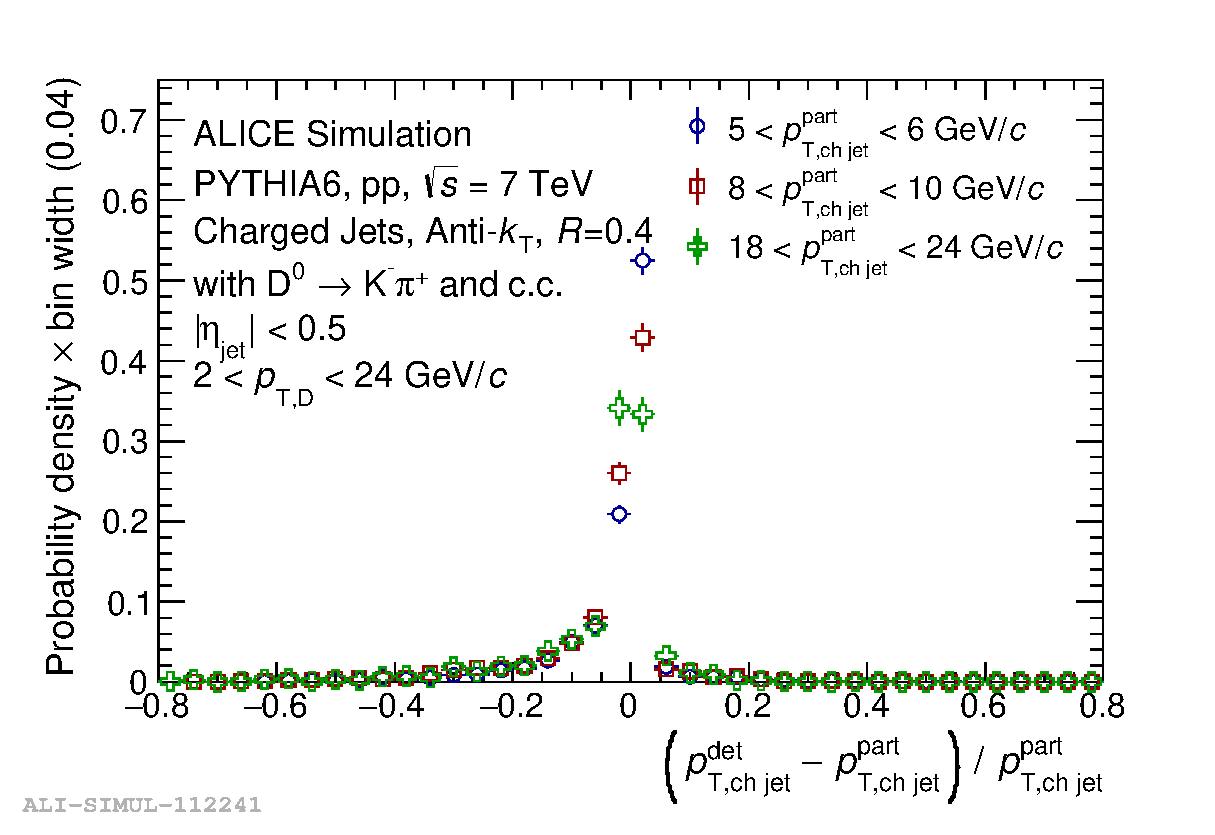
\includegraphics[width=\textwidth]{img/HQ16_Simulation_DetectorResponse}
\caption{\label{label}Figure caption for first of two sided figures.}
\end{minipage}\hspace{1pc}%
\begin{minipage}{.48\textwidth}
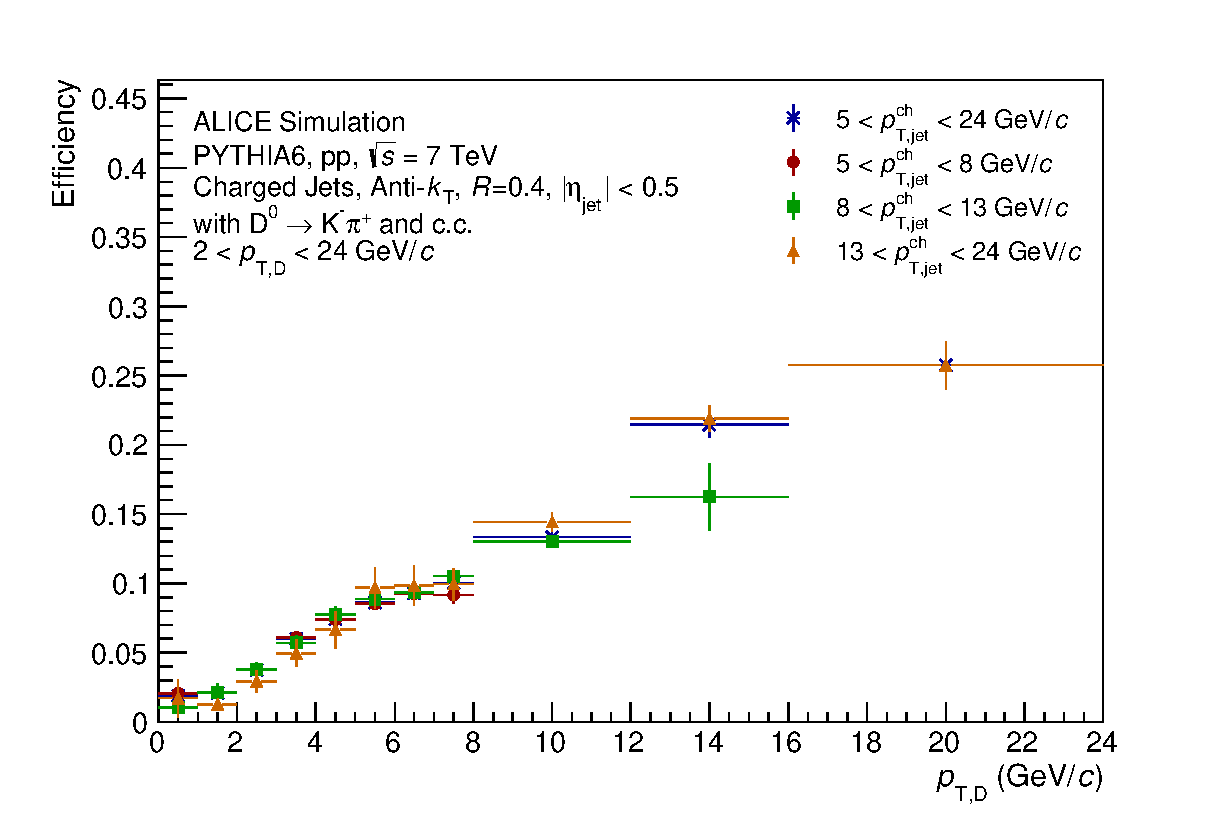
\includegraphics[width=\textwidth]{img/HQ16_Simulation_EfficiencyVsDPt}
\caption{\label{label}Figure caption for second of two sided figures.}
\end{minipage} 
\end{figure}

\begin{figure}[h]
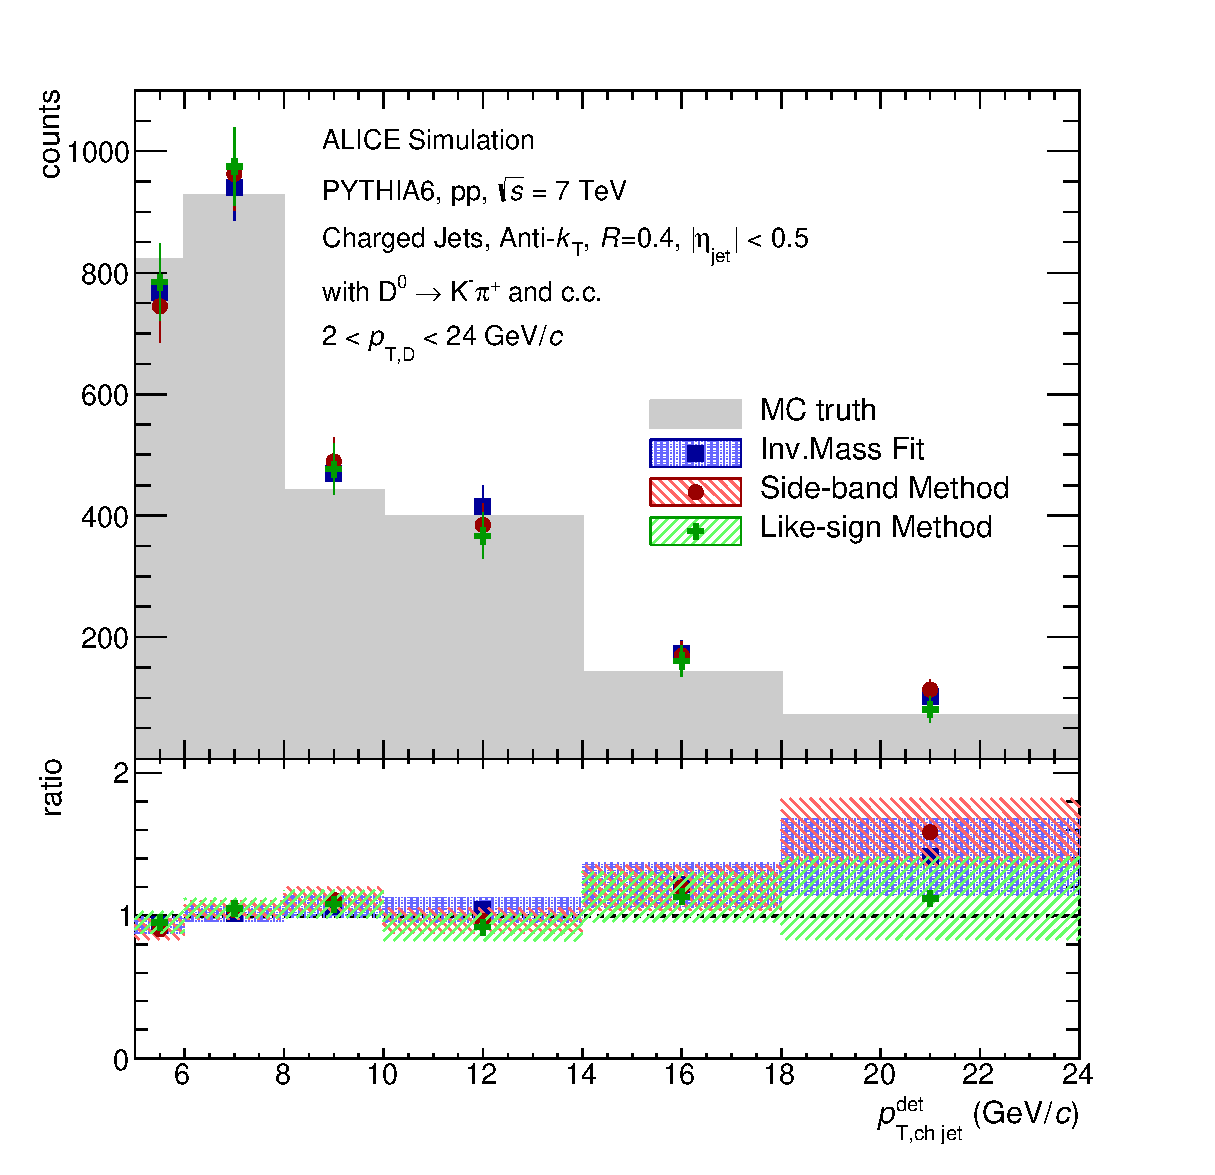
\includegraphics[width=.57\textwidth]{img/HQ16_Simulation_MethodComparison}\hspace{1pc}%
\begin{minipage}[b]{.39\textwidth}\caption{\label{label}Figure caption for a narrow figure where the caption is put at the side of the figure.}
\end{minipage}
\end{figure}

\section*{References}
\bibliography{biblio}{}
\bibliographystyle{iopart-num}

\end{document}


